\documentclass[a4paper,12pt]{article}
\usepackage{caption}
\usepackage{subcaption}
\usepackage{float}
\usepackage[T1]{fontenc}
\usepackage[italian]{babel}
\usepackage[utf8]{inputenc}
\input funzioni.sty
\input funzioni2.sty
\floatstyle{ruled}
\usepackage{hyperref}
\usepackage{graphicx}
\usepackage{amsmath}
\usepackage{amssymb}
\usepackage[width=125mm]{caption}
\usepackage{amsthm}
\usepackage{algorithm2e}
% Dimensione della pagina
\setlength{\oddsidemargin}{.3in}  % Distance from the left edge -1 inch 
\setlength{\textwidth}{145mm}     % Normal width of the text
\setlength{\topmargin}{.25in}     % Distance from top to PAGE'S HEAD -1 inch
\setlength{\textheight}{225mm}    % Height of the body of page
\setlength{\headheight}{0mm}      % Height of a box containing the head
\setlength{\parskip}{0.5mm}         % Extra vertical space before a paragraph
\setlength{\parindent}{9mm}       % Width of the indentation 
\linespread{1.12}                 % Line spacing        
\renewcommand{\floatpagefraction}{.9}

\begin{document}
\author{Stefano Mandelli}
\title{\bf \Huge Confronto delle prestazioni CPU-GPU per la simulazione di un reticolo di Ising-2D}
\date{}
\maketitle
\section{Scelta del modello}

Viene considerato un reticolo periodico di dimensione $d$, ad ogni cella del reticolo viene associato uno spin $s_i$ che può essere solo del tipo $s_i=\{+1, -1\}$.
La prima possibilità indica la direzione del dipolo magnetico, associato alla cella
i-esima del reticolo, verso l'alto la seconda verso il basso. Il sistema è descritto dall'Hamiltoniana di Ising
\newl{\mathcal{H} = -J\sum_{\langle i j \rangle}s_i s_j -h\sum_i s_i }
dove $h$ identifica un eventuale campo magnetico esterno. La prima sommatoria è fatta sui primi vicini e $J$ indica la costante di accoppiamento tra spin primi vicini.
Se $J>0$ stiamo descrivendo un sistema ferromagnetico, se $J<0$ uno anti-ferromagnetico. In questo caso viene considerato $J>0$ e tutte le simulazioni sono fatte considerando
il campo magnetico esterno nullo, quindi ad $h=0$.

Il modello di Ising (escluso il caso 1D) presenta una transizione di fase in prossimità di una \textit{temperatura critica} $T_c$. Per temperature maggiori di $T_c$ il sistema si comporta
in modo totalmente paramagnetico. Per temperature inferiori invece si ha un fenomeno di magnetizzazione spontanea.
Le grandezze fisiche che possono essere calcolate sono $\langle M \rangle$ e il calore specifico a volume costante $C_V$ che viene calcolato col teorema di fluttuazione-dissipazione.
La quantità interessente è $c_V = C_V / N$ dove $N$ è il numero totale di spin del reticolo. In questo modo la quantità
\newl{c_v = \frac{k_B\beta^2}{N}(\langle E^2 \rangle - \langle E \rangle^2)}
permette di confrontare i calori specifici per diversi size del reticolo.






\begin{figure}
	\centering
	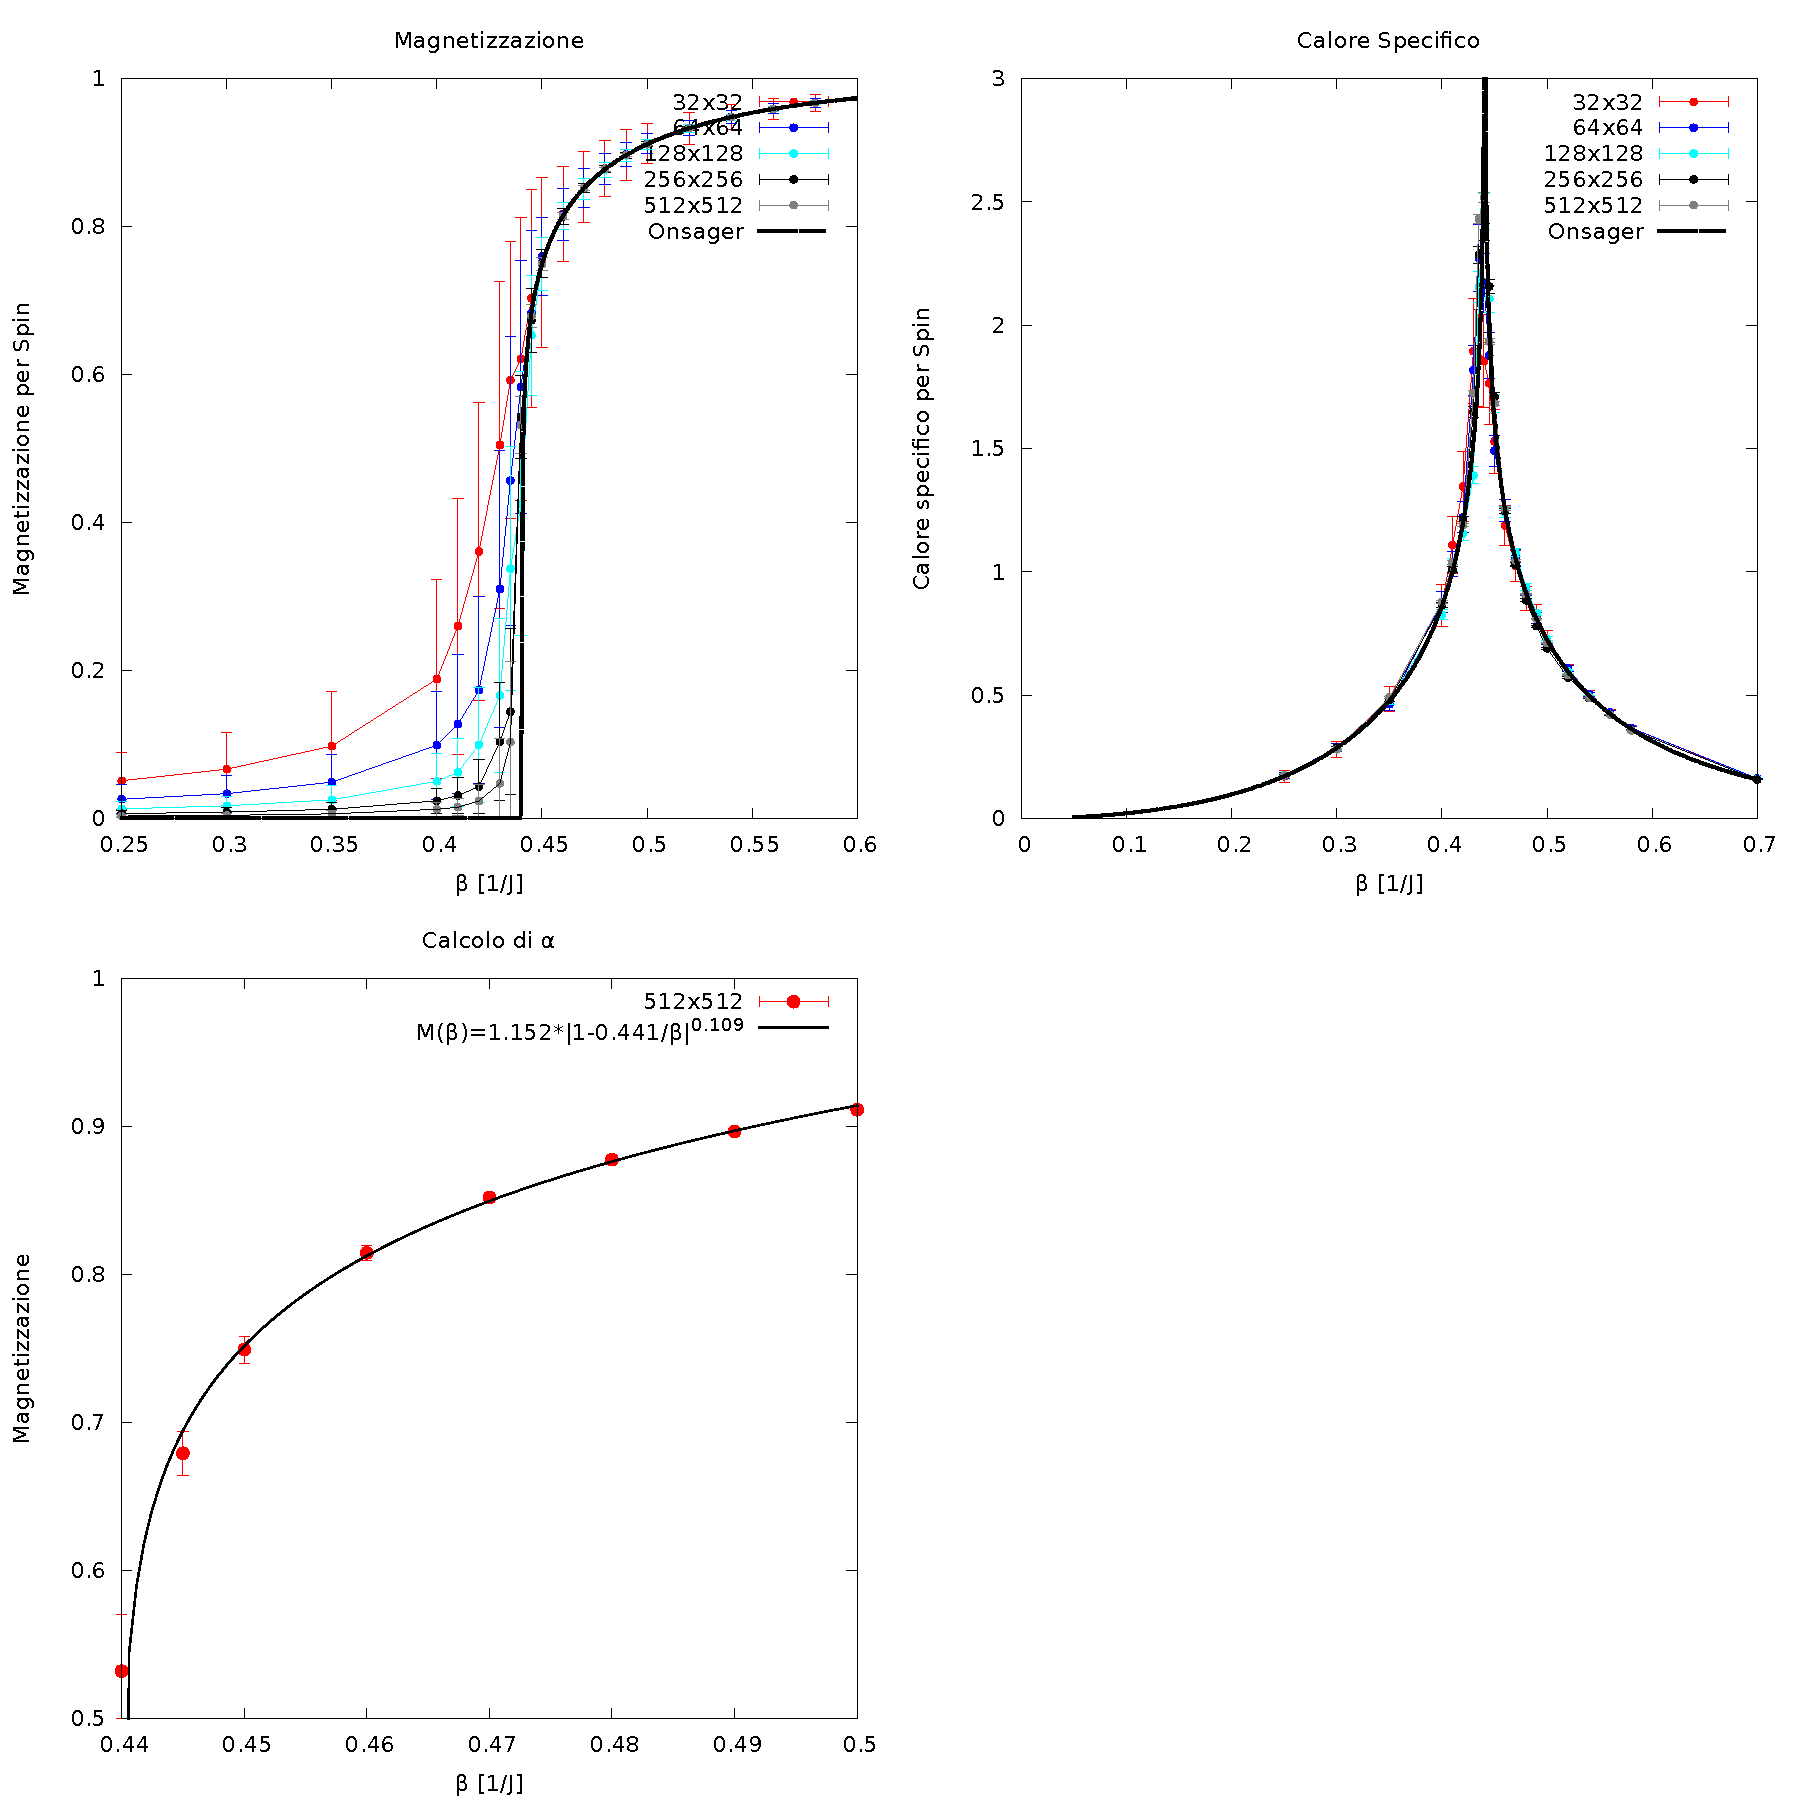
\includegraphics[width=120mm,angle=0,clip=]{../CPU/Result/Ising_Mag_Cv.pdf}
	\caption{Dati CPU}
	\label{figura:ratio}
\end{figure}

\begin{figure}
	\centering
	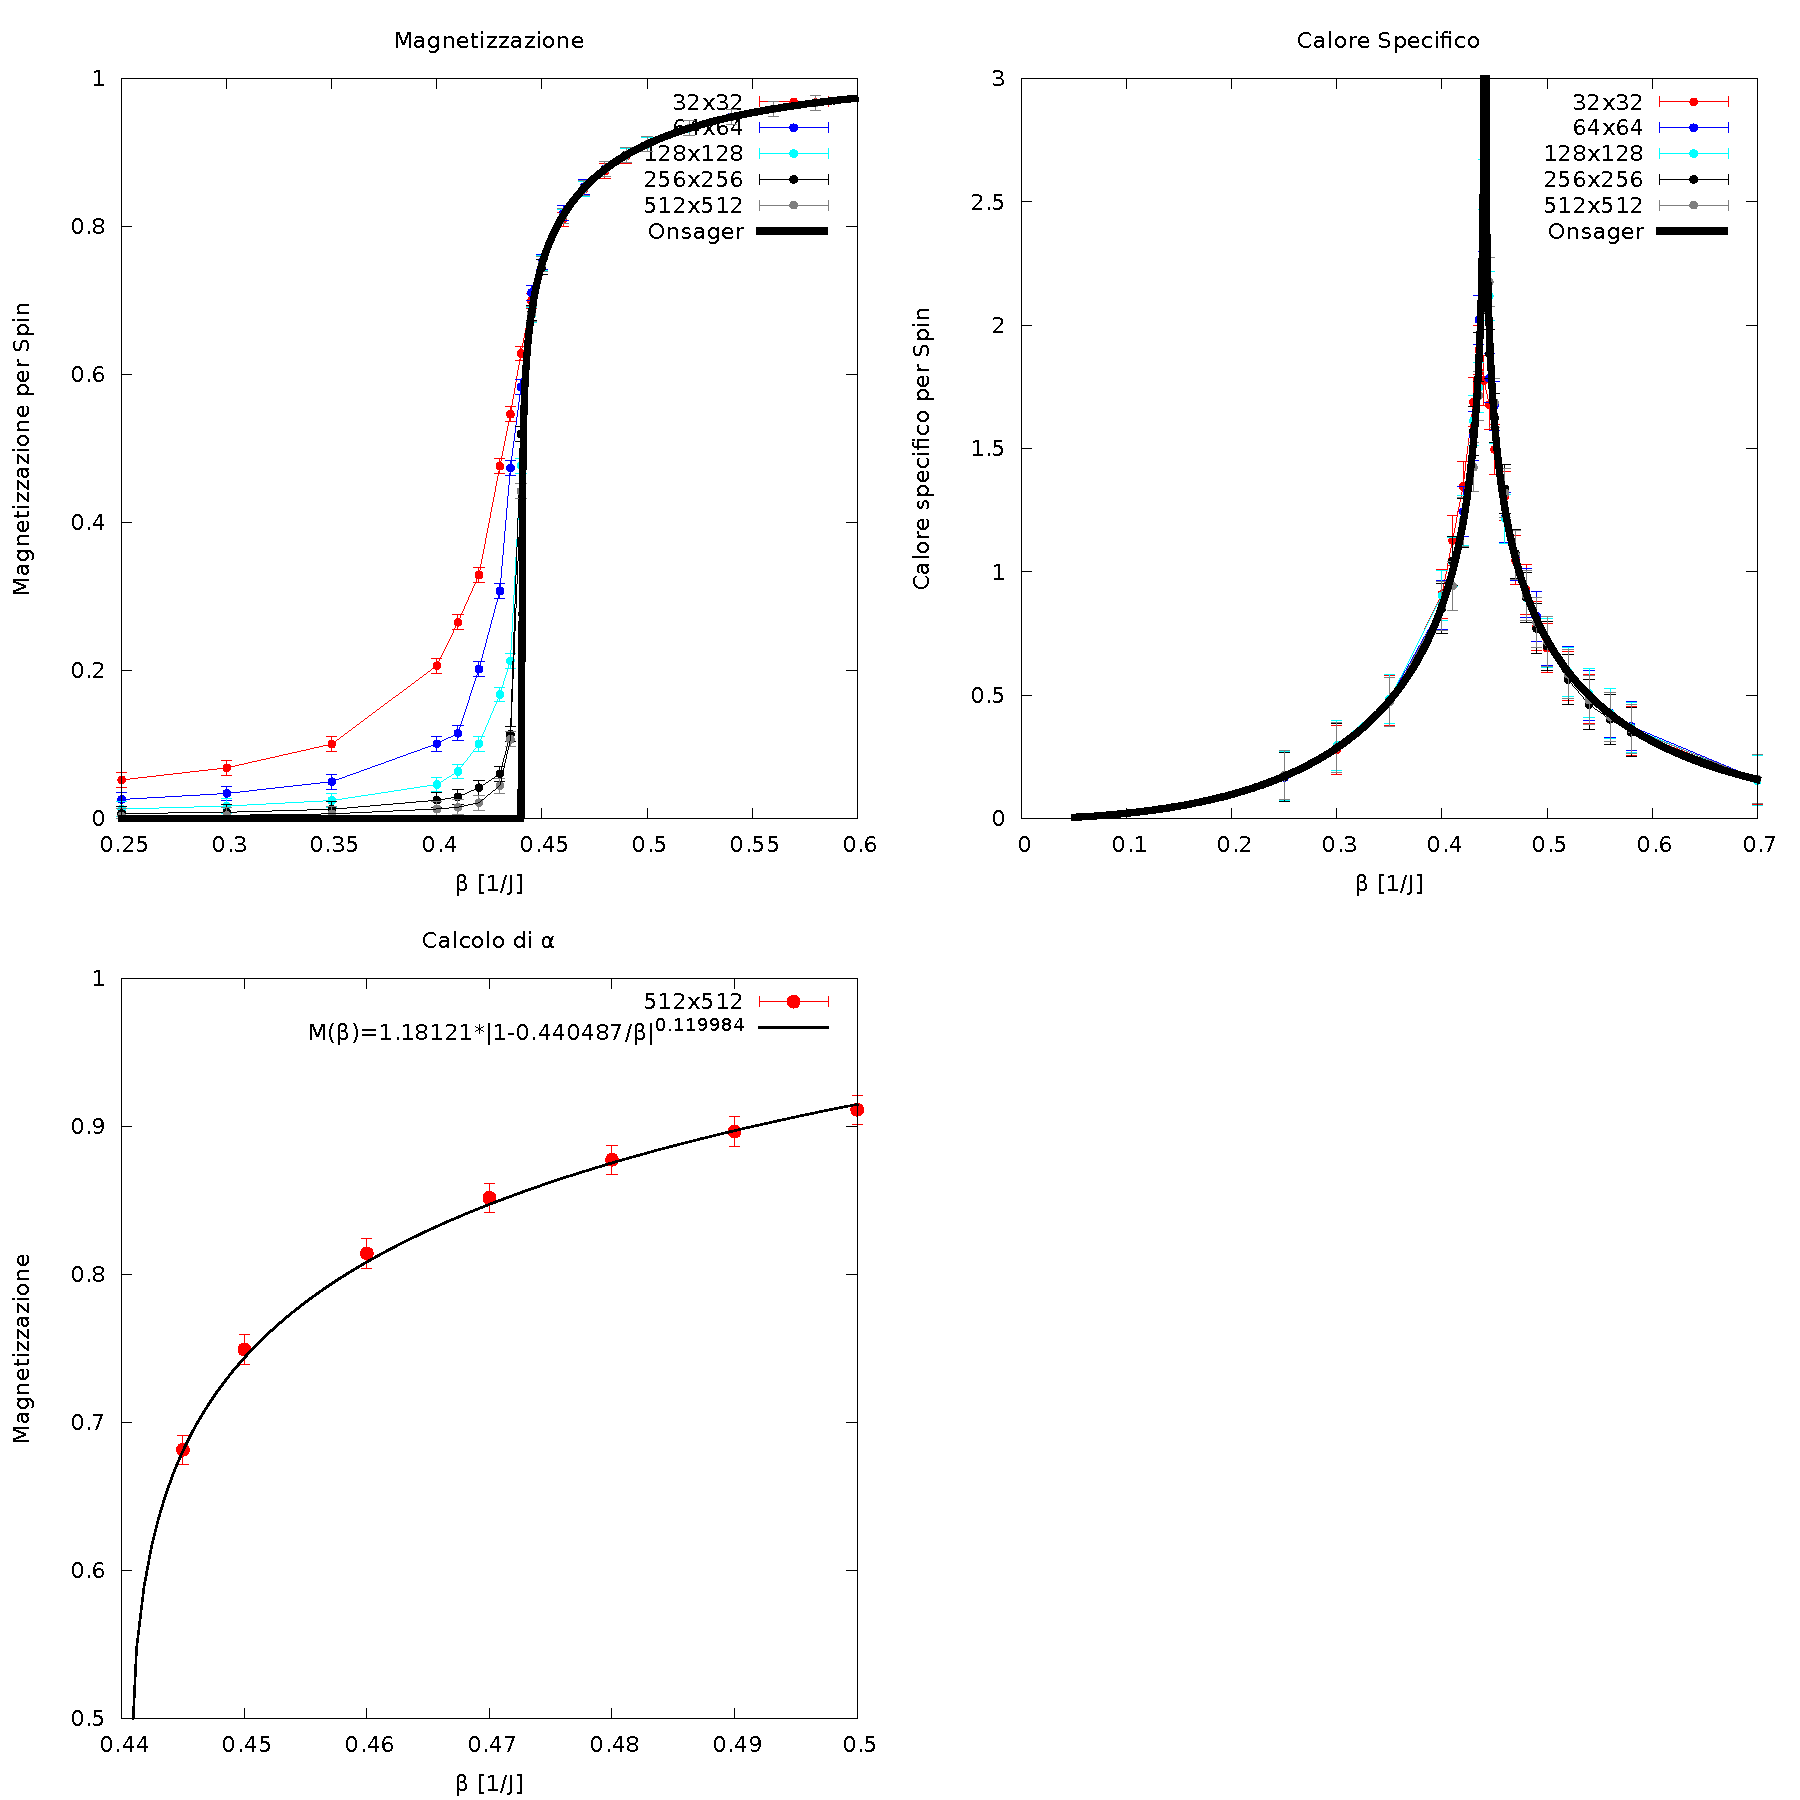
\includegraphics[width=120mm,angle=0,clip=]{../CUDA/Result/Res2/Ising_Mag_Cv.pdf}
	\caption{Dati GPU}
	\label{figura:ratio}
\end{figure}

\begin{figure}
	\centering
	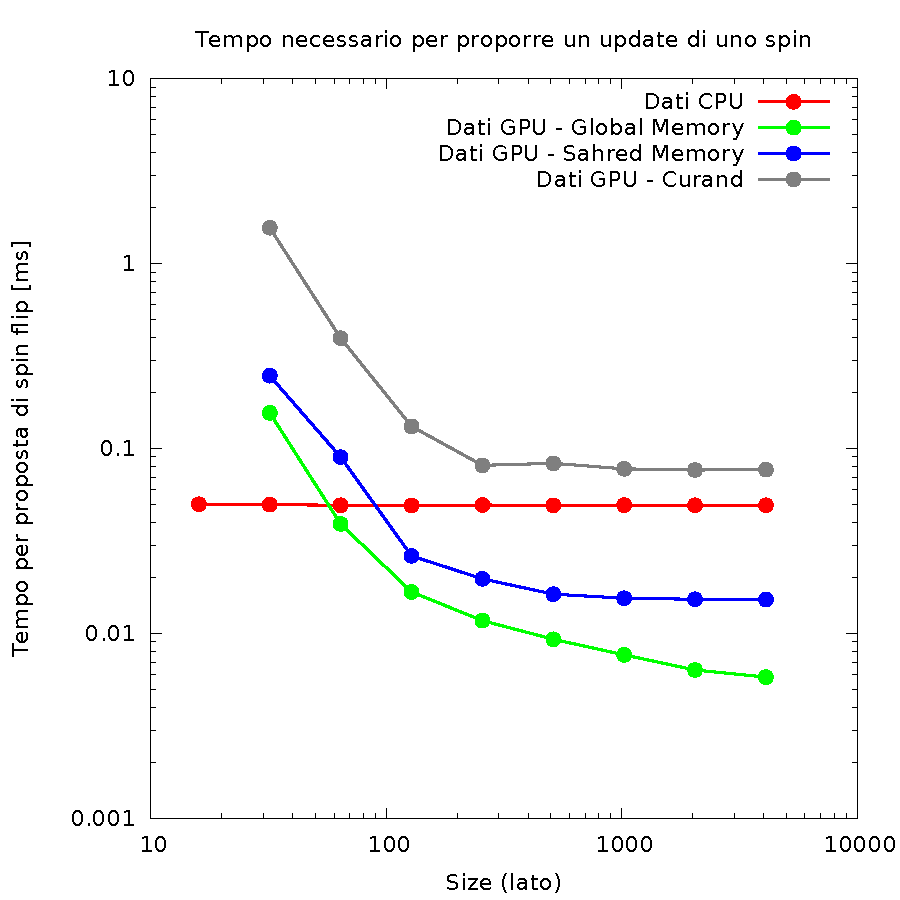
\includegraphics[width=120mm,angle=0,clip=]{../CPU-GPU-time.pdf}
	\caption{CPU/GPU}
	\label{figura:ratio}
\end{figure}





\section{Variabili termodinamiche di interesse}

\section{Il problema dei numeri pseudorandom}










\end{document}
